


\chapter{Экспериментальная часть}\label{exp}
%\addcontentsline{toc}{chapter}{4 Экспериментальная часть}

Оценка качества работы алгоритмов. Экспериментальное сравнение работы различных алгоритмов умножения матриц 
(зависимость времени выполнения от размерности матриц).

\section{Примеры работы}\label{examples}

На рисунках \ref{ris:w1}, \ref{ris:w2}, \ref{ris:w3}, \ref{ris:w4}, \ref{ris:w5} показаны примеры работы.

\begin{figure}[H]
    \center{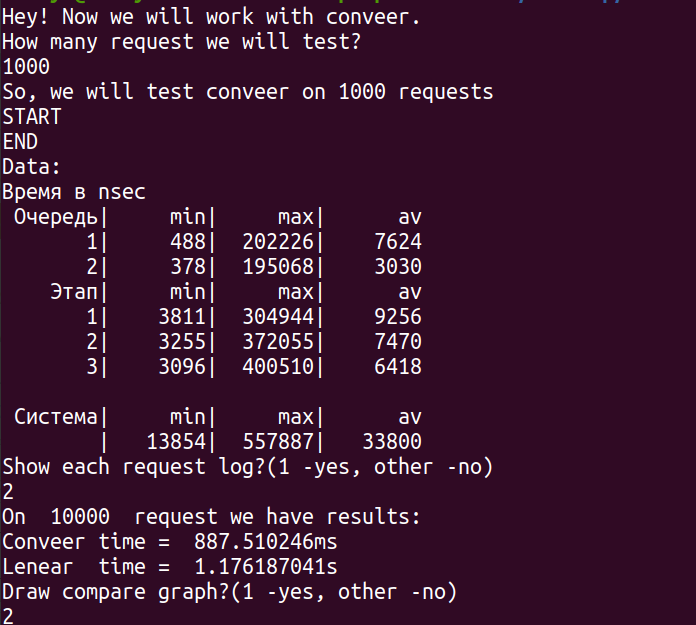
\includegraphics[scale=0.4]{w1}}
    \caption{Ручное тестирование: тест 1}
    \label{ris:w1}
\end{figure}

\begin{figure}[H]
    \center{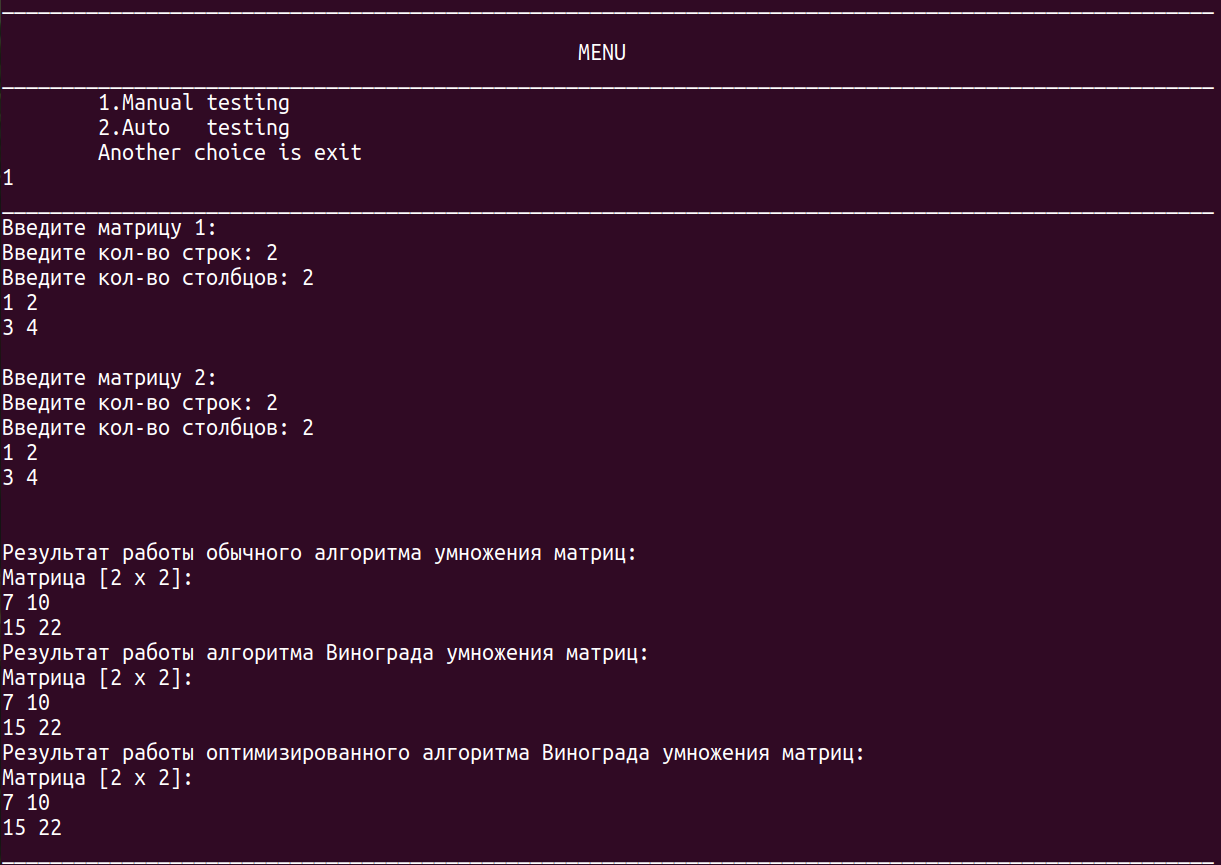
\includegraphics[scale=0.4]{w2}}
    \caption{Ручное тестирование: тест 2}
    \label{ris:w2}
\end{figure}

\begin{figure}[H]
    \center{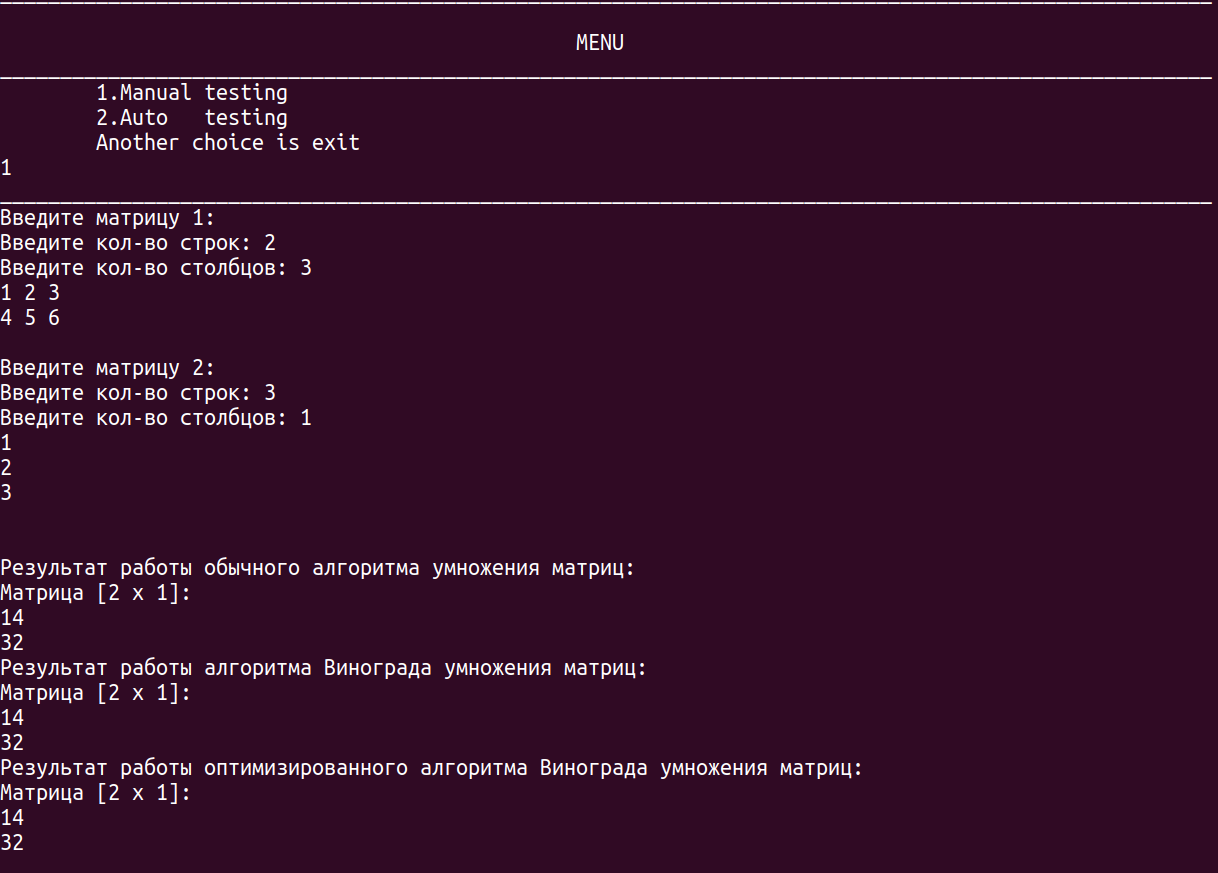
\includegraphics[scale=0.4]{w3}}
    \caption{Ручное тестирование: тест 3}
    \label{ris:w3}
\end{figure}

\begin{figure}[H]
    \center{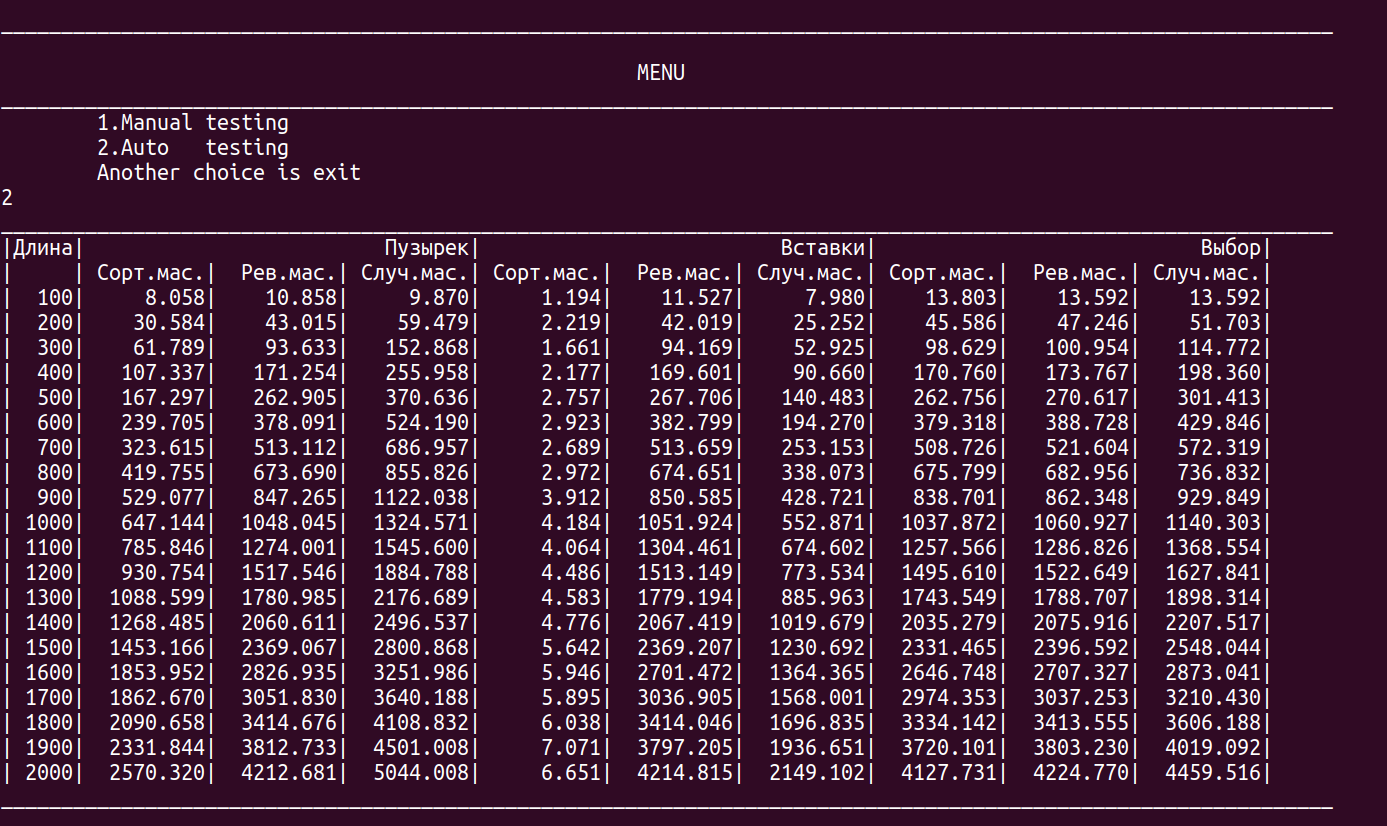
\includegraphics[scale=0.25]{w4}}
    \caption{Автотестирование}
    \label{ris:w4}
\end{figure}

\begin{figure}[H]
    \center{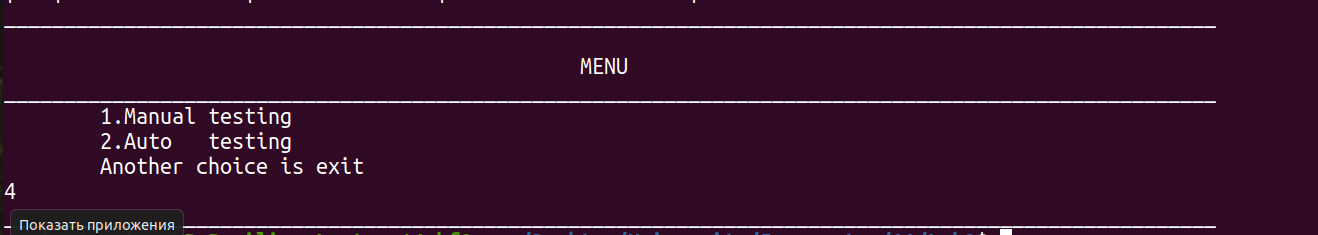
\includegraphics[scale=0.4]{w5}}
    \caption{Выход}
    \label{ris:w5}
\end{figure}
  
\section{Замеры времени}\label{experimentgraph}

На рисунках \ref{ris:graph1}, \ref{ris:graph2}, и \ref{ris:graph3}  и \ref{ris:graph4} показаны графические результаты сравнения исследуемых алгоритмов по времени. 

\begin{figure}[H]
    \center{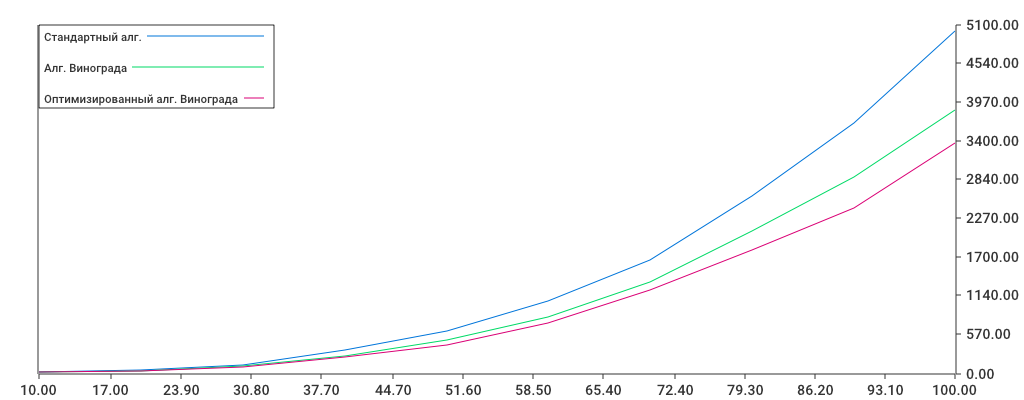
\includegraphics[scale=0.4]{../Lab2/output.png}}
    \caption{Сравнение 3 исследуемых алгоритмов по времени (размер матрицы четный)}
    \label{ris:graph1}
\end{figure}

\begin{figure}[H]
    \center{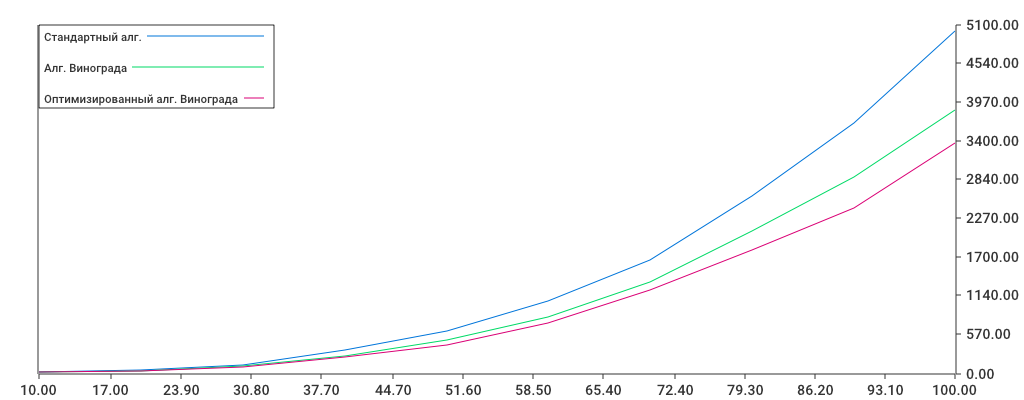
\includegraphics[scale=0.4]{../Lab2/output2.png}}
    \caption{Сравнение 3 исследуемых алгоритмов по времени (размер матрицы нечетный)}
    \label{ris:graph2}
\end{figure}

\begin{figure}[H]
    \center{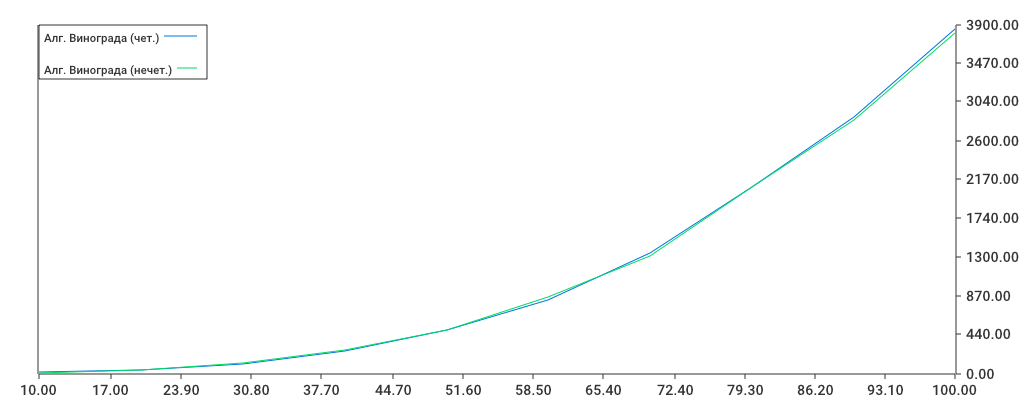
\includegraphics[scale=0.4]{../Lab2/output3.png}}
    \caption{Сравнение алгоритма Винограда четные и нечетные размеры матриц}
    \label{ris:graph3}
\end{figure}

\begin{figure}[H]
    \center{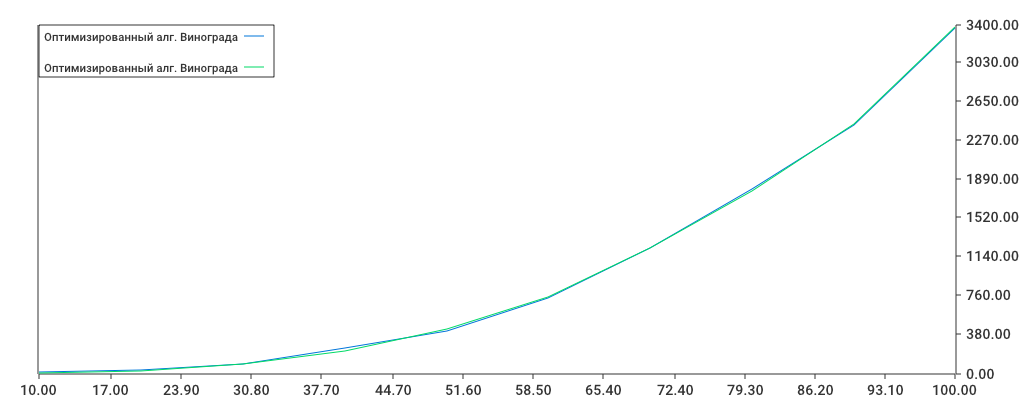
\includegraphics[scale=0.4]{../Lab2/output4.png}}
    \caption{Сравнение оптимизированного алгоритма Винограда четные и нечетные размеры матриц}
    \label{ris:graph4}
\end{figure}

\section{Сравнительный анализ алгоритмов}\label{comparepart}


Из проведенных замеров видно, что оптимизация алгоритма Винограда получилась эффективнее по времени, чем сам алгоритм Винограда, следовательно 
предположение, сделанное из трудоемкостей алгоритмов, верно. Самым выгодным по времени алгоритмом из исследуемых является оптимизированный
алгоритм Винограда. Самым медленным из исследуемых алгоритмов оказался стандартный алгоритм, как и было предположено. Различия в скорости 
при обработке матриц четных и нечетных размеров незначительны, как это видно из графиков \ref{ris:graph3} и \ref{ris:graph4}, как для 
обычного алгоритма Винограда, так и для оптимизированного.


\section{Вывод экспериментальной части}\label{experimentresult}

Таким образом, подтвердилось предположение, что самый эффективный алгоритм из рассматриваемых в работе - оптимизированный алгоритм Винограда.
Различия в скорости при обработке матриц четных и нечетных размеров незначительны, как для обычного алгоритма Винограда, так и
для оптимизированного.



\chapter{Заключение}\label{exit}

В данной работе были изучены алгоритмы умножения матриц. 
Получены практические навыки реализации исследуемых алгоритмов. Была подсчитана трудоемкость исследуемых алгоритмов. 
Проведён сравнительный анализ алгоритмов по времени и трудоемкости. 
Показано, что наименее трудоемкий и наименее затратный по времени при
больших размерах матриц алгоритм Винограда оптимизированный.
Экспериментально подтверждены различия в эффективности алгоритмов с указанием лучших и худших случаев. 
Цель работы достигнута, решены поставленные задачи. 
Показано, что наименее трудоемкий и наименее затратный по времени при
больших размерах матриц алгоритм Винограда оптимизированный.
Получены практические навыки реализации алгоритмов Винограда и стандартного алгоритма, а также проведена исследовательская работа 
по оптимизации и вычислении трудоемкости алгоритмов.
